\documentclass[10pt]{article}

\usepackage{fullpage}
\usepackage[normalem]{ulem} % For strikethrough font
\usepackage{graphicx}
\graphicspath{ {./} }
\usepackage{xcolor}
\usepackage{listings}
\usepackage{float}
\usepackage[T1]{fontenc}
\usepackage{sourcecodepro}
\usepackage[T1]{fontenc}
\lstset{basicstyle=\footnotesize\ttfamily}
\usepackage[sfdefault]{universalis} % load the font and set it to default

\definecolor{mGreen}{rgb}{0,0.6,0}
\definecolor{mGray}{rgb}{0.5,0.5,0.5}
\definecolor{mPurple}{rgb}{0.58,0,0.82}
\definecolor{backgroundColour}{rgb}{0.95,0.95,0.92}
\lstset{
	basicstyle=\small\selectfont\ttfamily
}
\lstdefinestyle{CStyle}{                 
	backgroundcolor=\color{backgroundColour},   
	commentstyle=\color{mGreen},
	keywordstyle=\color{magenta},
	numberstyle=\tiny\color{mGray},
	stringstyle=\color{mPurple},
	breakatwhitespace=false,         
	breaklines=true,                 
	captionpos=b,                    
	keepspaces=true,                 
	numbers=left,                    
	numbersep=5pt,                  
	showspaces=false,                
	showstringspaces=false,
	showtabs=false,                  
	tabsize=2,
	language=C
}

\title{LED Sequence V3.0}
% Name, netid
\author{Khaled Mustafa Anwar}

\begin{document}
\maketitle

\section{Introduction}
This task controls the LED lighting sequence according to button pressing, and alternates between 5 different blinking states.

\section{Flowchart}

\subsubsection{LED Sequence Application}
\begin{figure}[H]
	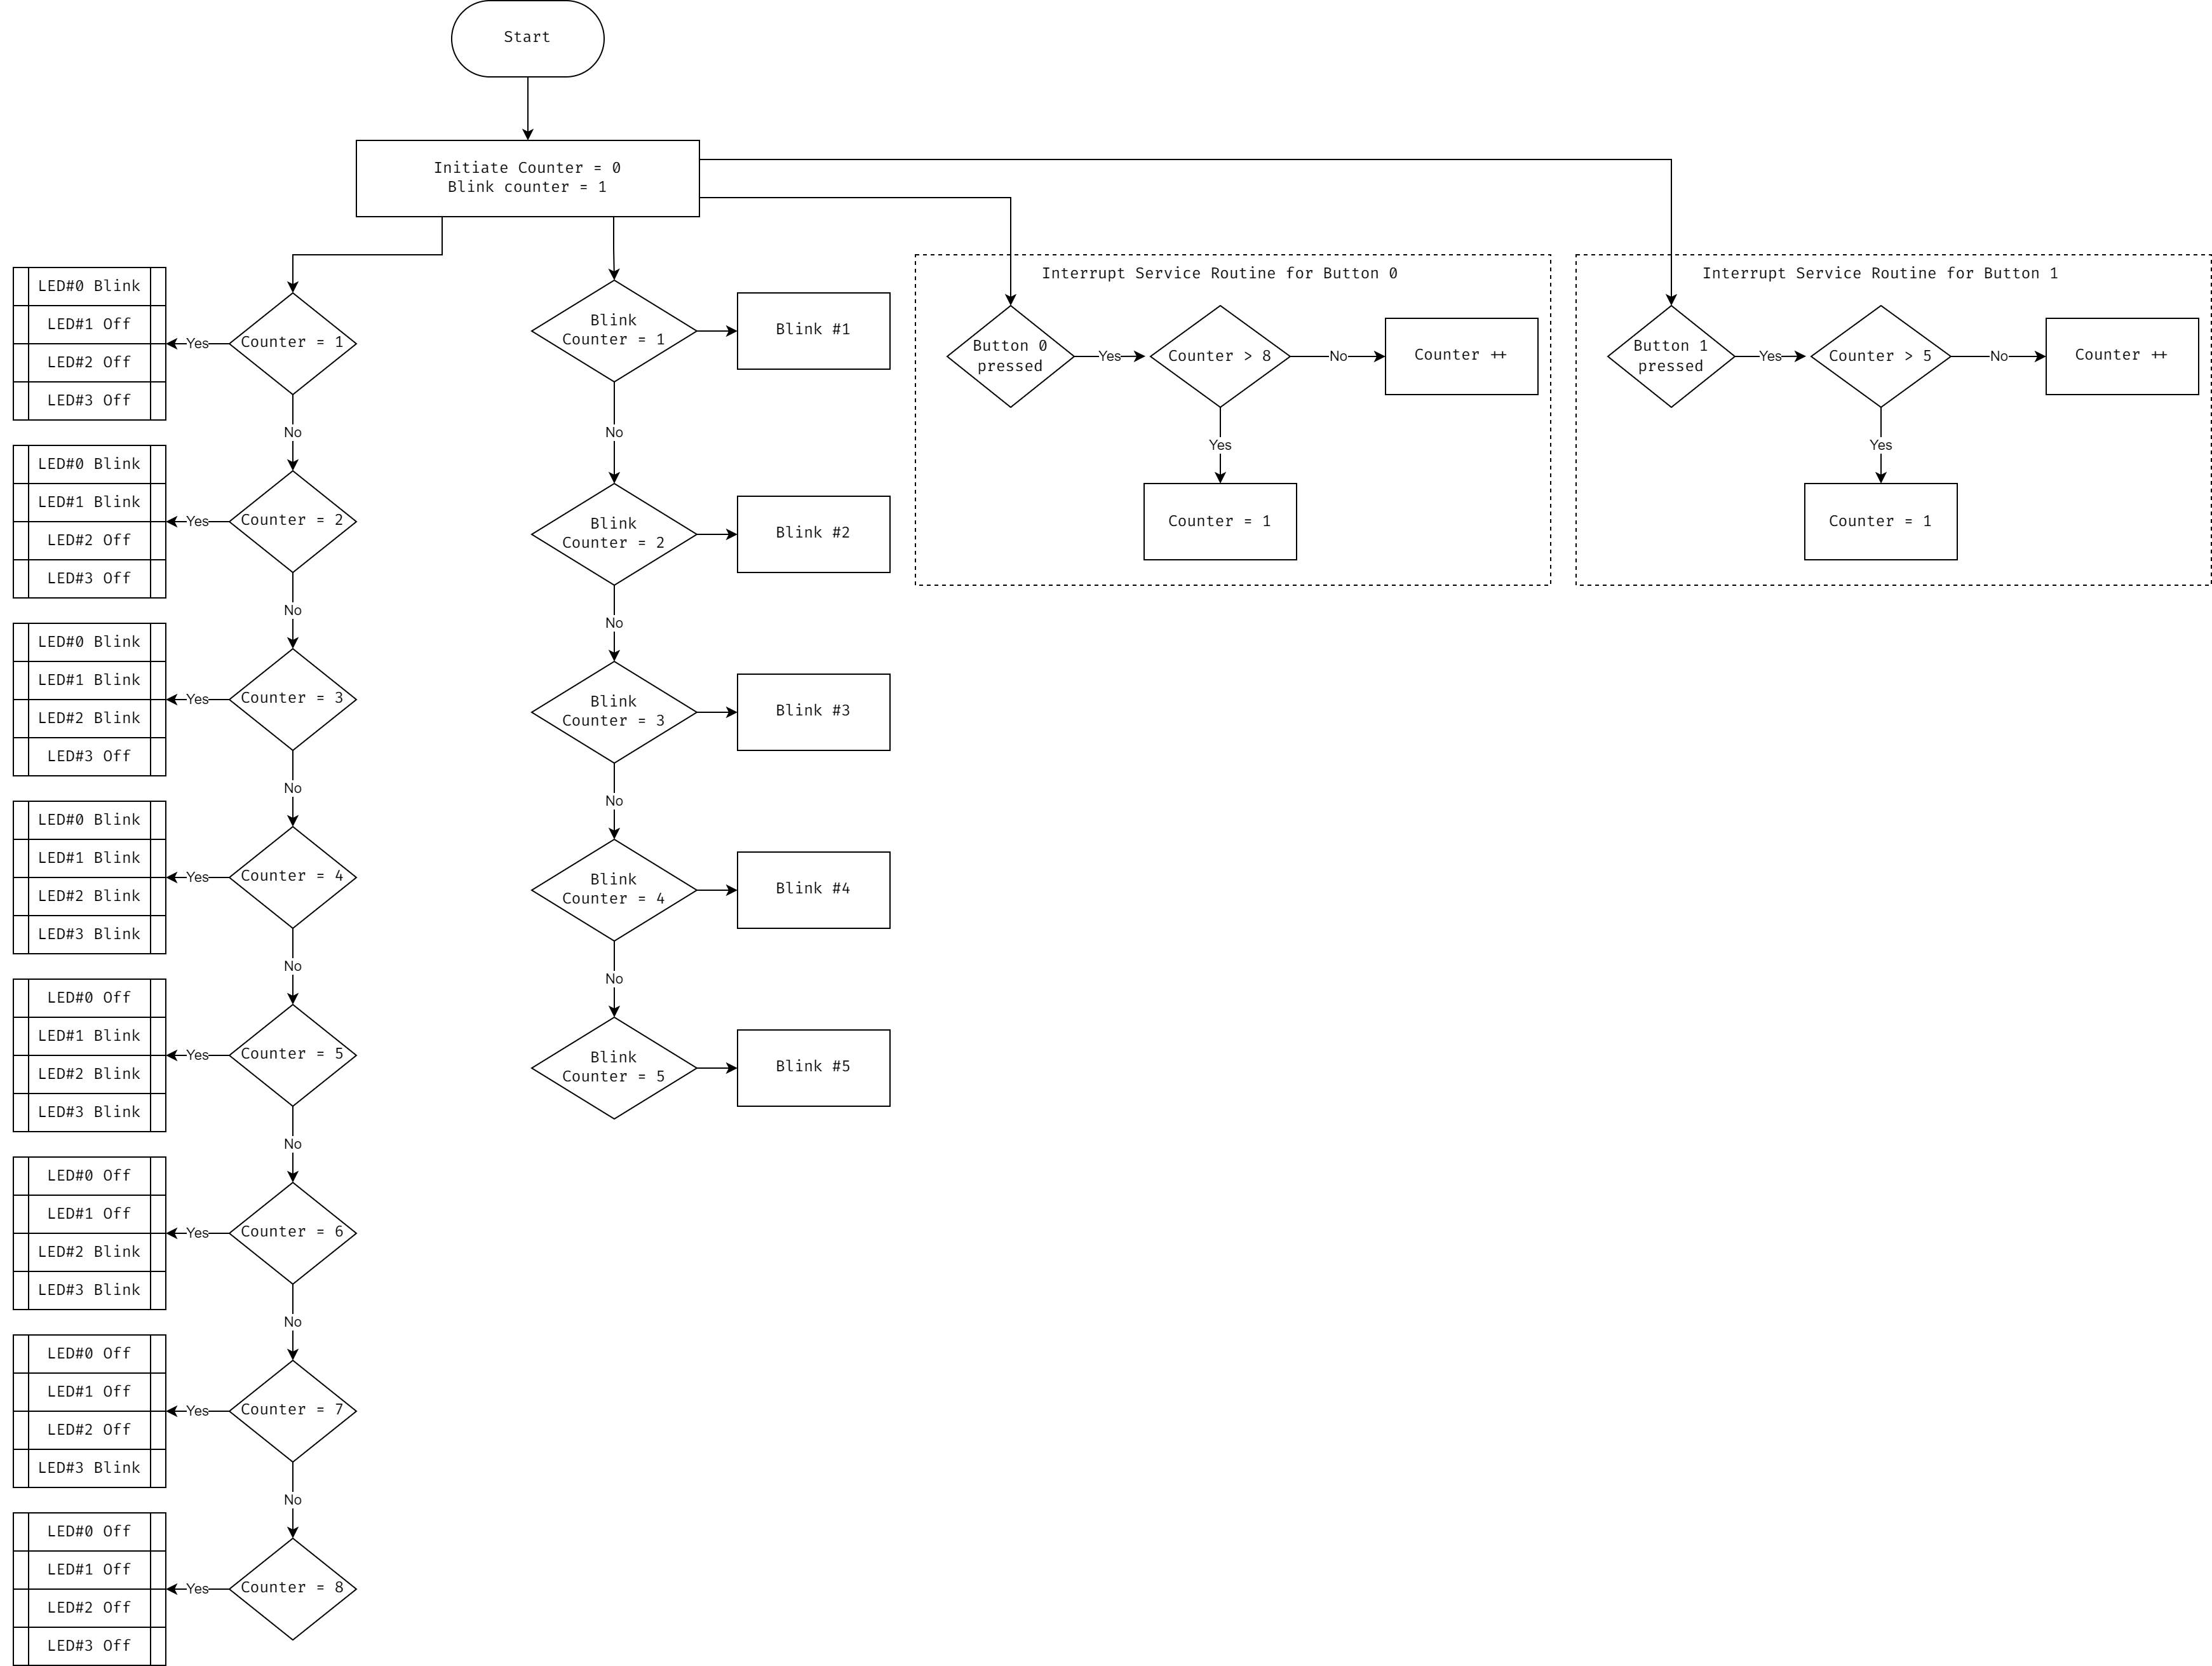
\includegraphics[width=14cm]{led-sequence_v_3_0}
	\centering
\end{figure}

\subsubsection{DIO flowchart}
\begin{figure}[H]
	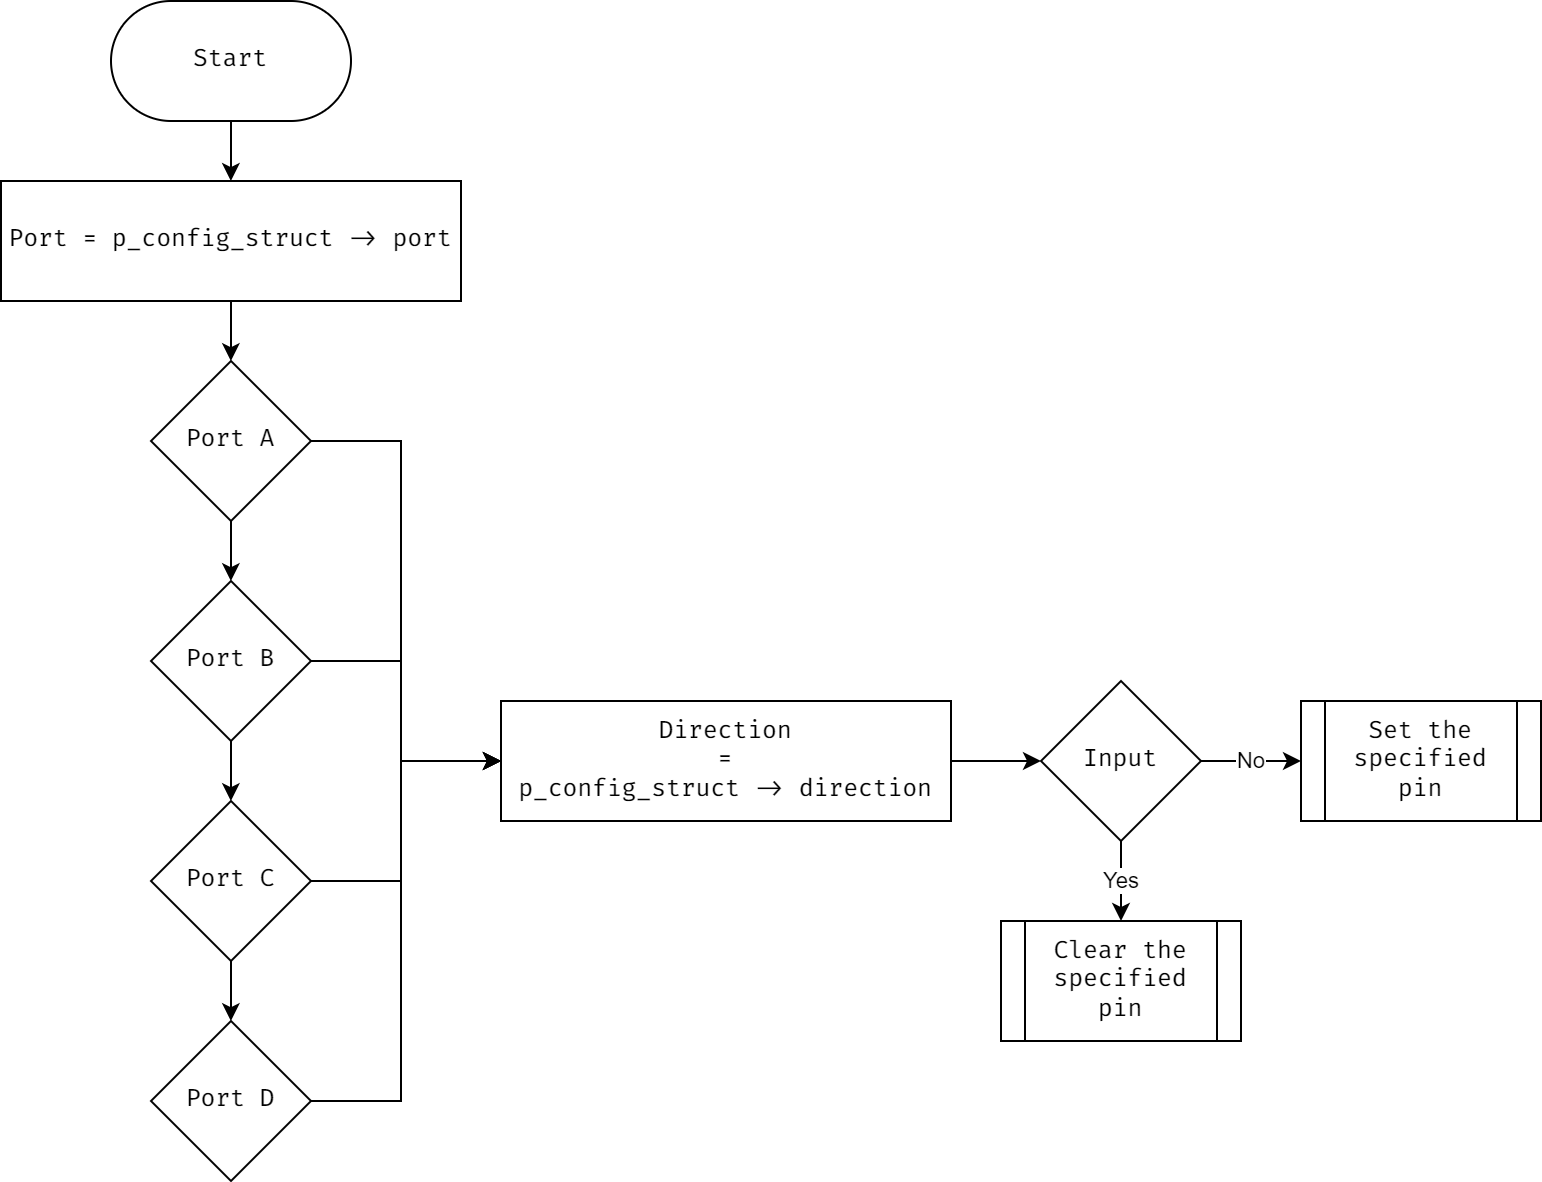
\includegraphics[width=14cm]{dio_flowchart}
	\centering
\end{figure}

\subsubsection{External interrupt flowchart}
\begin{figure}[H]
	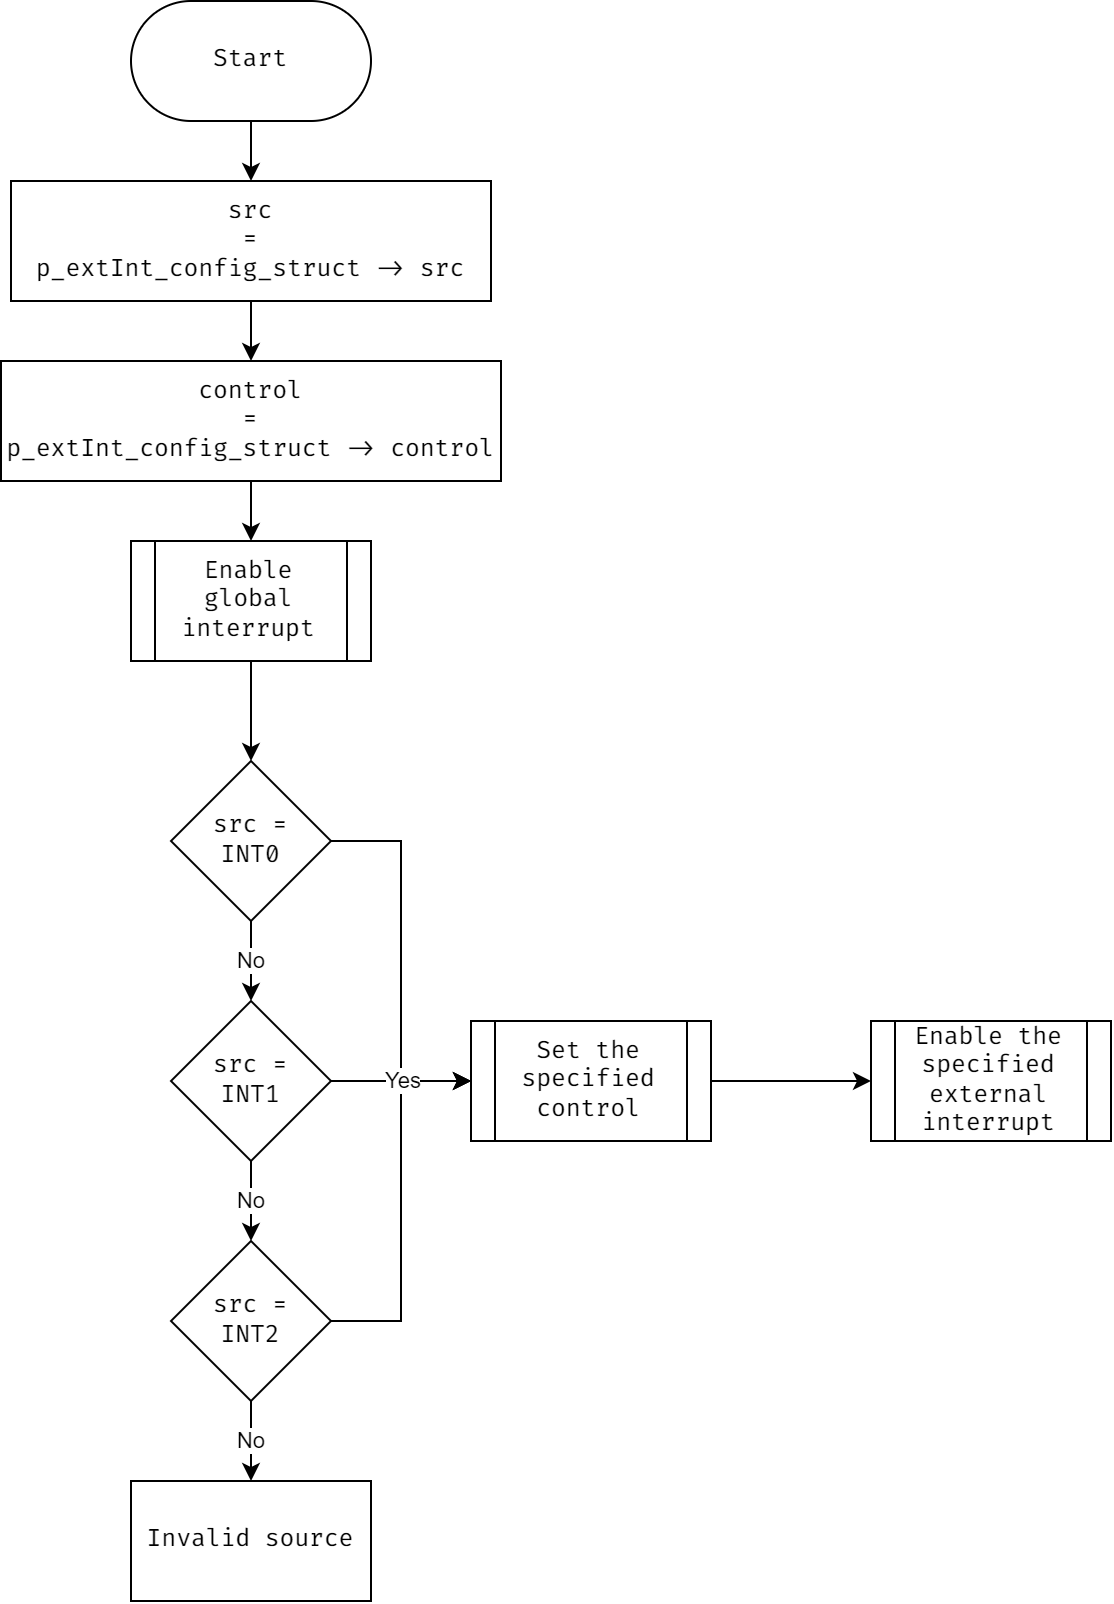
\includegraphics[width=14cm]{external_interrupt_flowchart}
	\centering
\end{figure}

\subsubsection{Push button flowchart}
\begin{figure}[H]
	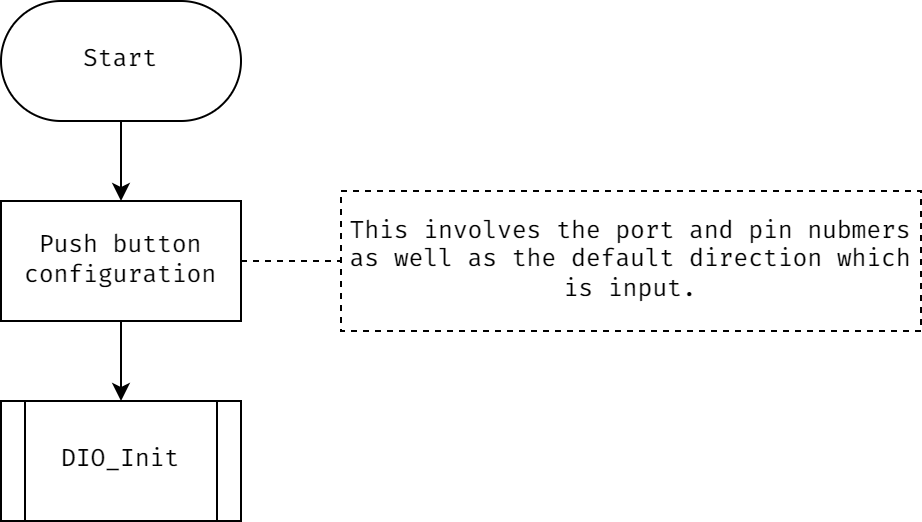
\includegraphics[width=14cm]{push_button_flowchart}
	\centering
\end{figure}

\subsubsection{LED flowchart}
\begin{figure}[H]
	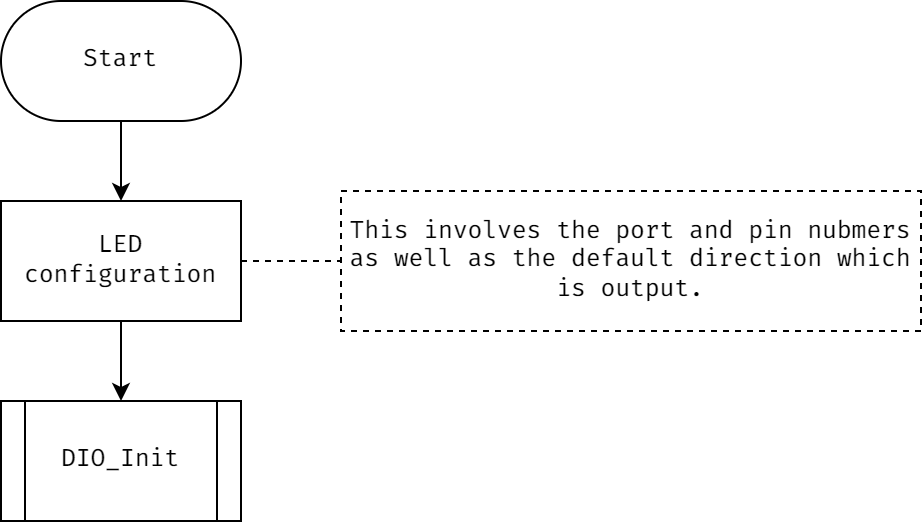
\includegraphics[width=14cm]{led_init_flowchart}
	\centering
\end{figure}

\subsubsection{Timer initialization flowchart}
\begin{figure}[H]
	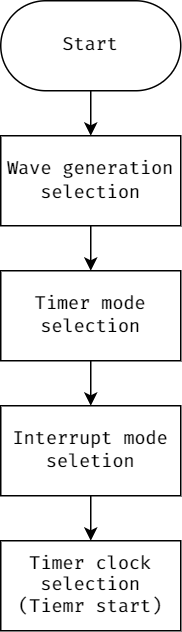
\includegraphics[width=3cm]{timer-init}
	\centering
\end{figure}

\section{Layered architecture}

\begin{figure}[H]
	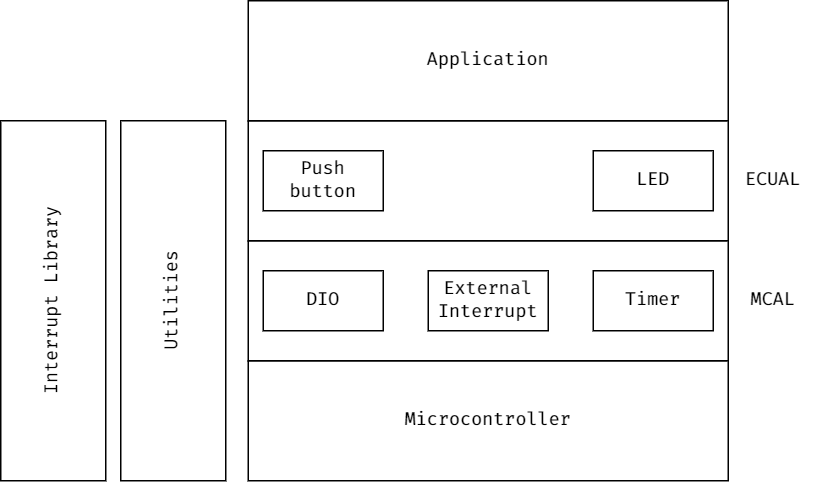
\includegraphics[width=14cm]{layered-arhictecture_v_3_0}
	\centering
\end{figure}

\section{Application Binary Interface (API)}
\subsection{Microcontroller Architecture Layer (MCAL)}
\subsubsection{DIO}
\begin{lstlisting}[style=CStyle,escapeinside=``]
	/**
	* @enum EN_DIO_ERROR_STATE
	* @brief Defines the state of DIO functions.
	*/
	typedef enum EN_DIO_ERROR_STATE {
		DIO_SUCCESS = 0, DIO_PORT_INVALID, DIO_DIRECTION_INVALID, DIO_PIN_INVALID
	}EN_DIO_ERROR_STATE;
	
	/**
	* @enum EN_DIO_DIRECTION
	* @brief Specifies the state of the pin.
	*/
	typedef enum EN_DIO_DIRECTION {
		DIO_INPUT = 0, DIO_OUTPUT
	}EN_DIO_DIRECTION;
	
	/**
	* @enum EN_DIO_PIN
	* @brief Specifies the number of pin.
	*/
	typedef enum EN_DIO_PIN {
		PIN0 = 0, PIN1, PIN2, PIN3, PIN4, PIN5, PIN6, PIN7, PIN8
	}EN_DIO_PIN;
	
	/**
	* @enum EN_DIO_PORT
	* @brief Specifies the port number.
	* the port number and returns the address of the corresponding port.
	*/
	typedef enum EN_DIO_PORT {
		PORT_A = 0, PORT_B, PORT_C, PORT_D
	}EN_DIO_PORT;
	
	/**
	* @enum EN_DIO_LEVEL
	* @brief Specifies the level of the pin.
	*/
	typedef enum EN_DIO_LEVEL {
		DIO_LOW = 0, DIO_HIGH
	}EN_DIO_LEVEL;
	
	/**
	* @struct DIO_Init_t
	* @brief Holds the configuration of a specific pin of a port.
	* @var DIO_Init_t::port
	* Member 'port' sets the port to be configured.
	* @var DIO_Init_t::pin
	* Member 'pin' sets the pin to be configured.
	* @var DIO_Init_t::direction
	* Member 'direction' sets the direction of the pin.
	* @var DIO_Init_t::pin_value
	* Member 'pin_value; contains the value of the pin when it's configured as input mode.
	* @var DIO_Init_t::port_value
	* Member 'port_value' contains the value to be written to the port register if the pin is configured as output.
	*/
	typedef struct DIO_Init_t {
		EN_DIO_PORT port;
		EN_DIO_PIN pin;
		EN_DIO_DIRECTION direction;
		union {
			uint8 pin_value;
			uint8 port_value;
		};
	}DIO_Init_t;
	
	/**
	* @brief Initializes the direction of the specified pin.
	* @param[in] p_config_struct Address of the configuration structure.
	* @return DIO_PORT_INVALID Port in invalid.
	* @return DIO_SUCCESS The pin initialization is a success.
	*/
	EN_DIO_ERROR_STATE DIO_Init(DIO_Init_t *p_config_struct);
	
	`\newpage`
	
	/**
	* @brief Reads the state of a specific pin.
	* @param[in] p_config_struct Address of the configuration structure.
	* @return DIO_PORT_INVALID Port is invalid.
	* @return DIO_DIRECTION_INVALID Reading from a pin that is configured as output.
	* @return DIO_SUCCESS The read operation is a success.
	*/
	EN_DIO_ERROR_STATE DIO_ReadPin(DIO_Init_t *p_config_struct);
	
	/**
	* @brief Write a specific level to a specified pin.
	* @param[in] p_config_struct Address of the configuration structure.
	* @return DIO_PORT_INVALID Port is invalid.
	* @return DIO_DIRECTION_INVALID Writing to a pin that is configured as input.
	* @return DIO_SUCCESS The write operation is a success.
	*/
	EN_DIO_ERROR_STATE DIO_WritePin(DIO_Init_t *p_config_struct);
	
	/**
	* @brief Toggles the current level of a pin.
	* @param[in] p_config_struct Address of the configuration structure.
	*  @return DIO_PORT_INVALID Port is invalid.
	* @return DIO_DIRECTION_INVALID Toggle a pin that is configured as input.
	* @return DIO_SUCCESS The toggle operation is a success.
	*/
	EN_DIO_ERROR_STATE DIO_TogglePin(DIO_Init_t *p_config_struct);
\end{lstlisting}

\subsubsection{External Interrupts}
\begin{lstlisting}[style=CStyle,escapeinside=``]
	/**
	* @enum EN_INT_ERROR_STATE
	* @brief Specifies the state of DIO functions.
	*/
	typedef enum EN_INT_ERROR_STATE {
		INT_SUCCESS = 0, INT_GLOBAL_INT_NOT_SET, INT_INVALID_CONTROL, INT_INVALID_EXTERNAL_SRC
	}EN_INT_ERROR_STATE;
	
	/**
	* @enum EN_EXT_INT_SENSE_CONTROL
	* @brief Specifies the triggering mechanism for the external interrupts.
	*/
	typedef enum EN_EXT_INT_SENSE_CONTROL {
		LOW_LEVEL = 0, ANY_LOGIC_CHANGE, FALLING_EDGE, RISING_EDGE
	}EN_EXT_INT_SENSE_CONTROL;
	
	/**
	* @enum EN_EXT_INTERRUPT_SRC
	* @brief Specifies the external interrupts source.
	*/
	typedef enum EN_EXT_INTERRUPT_SRC {
		INT0 = 0, INT1, INT2
	}EN_EXT_INTERRUPT_SRC;
	
	/**
	* @enum EN_EXT_INTERRUPT_BITS
	* @brief Control sense configuration bits.
	*/
	typedef enum EN_EXT_INTERRUPT_BITS {
		ISC00 = 0, ISC01, ISC10, ISC11, ISC2 = 6
	}EN_EXT_INTERRUPT_BITS;
	
	/**
	* @struct INT_ExtInit_t
	* @brief Holds the configuration of external interrupts.
	* @var INT_ExtInit_t::src
	* Member 'src' specifies the external source of the interrupt.
	* @var INT_ExtInit_t::control
	* Member 'control' specifies how the external pin gets triggered.
	*/
	typedef struct INT_ExtInit_t {
		EN_EXT_INTERRUPT_SRC src;
		EN_EXT_INT_SENSE_CONTROL control;
	}INT_ExtInit_t;
	
	/**
	* @brief Enables and sets the sense control of the external interrupt.
	* @param ext_int_config_struct
	* @return INT_INVALID_EXTERNAL_SRC
	* @return INT_SUCCESS
	*/
	EN_INT_ERROR_STATE INT_ExtInterruptInit(INT_ExtInit_t *ext_int_config_struct);
	
	/**
	* @brief Enables external interrupt 0.
	* @return INT_GLOBAL_INT_NOT_SET
	* @return INT_SUCCESS
	*/
	EN_INT_ERROR_STATE INT_EnableINT0();
	
	/**
	* @brief Enables external interrupt 1.
	* @return INT_GLOBAL_INT_NOT_SET
	* @return INT_SUCCESS
	*/
	EN_INT_ERROR_STATE INT_EnableINT1();
	
	/**
	* @brief Enables external interrupt 2.
	* @return INT_GLOBAL_INT_NOT_SET
	* @return INT_SUCCESS
	*/
	EN_INT_ERROR_STATE INT_EnableINT2();
	
	`\newpage`
	
	/**
	* @brief Controls the triggering mechanism of INT1 and INT0.
	* Interrupt 0 sense control.
	* | ISC01 Bit 3 | ISC00 Bit 2 | Description                       |
	* |-------------|-------------|-----------------------------------|
	* | 0           | 0           | INT0 triggered on low level.      |
	* | 0           | 1           | Any logic change triggers.        |
	* | 1           | 0           | Falling edge generates interrupt. |
	* | 1           | 1           | Rising edge generates interrupt.  |
	* Interrupt 1 sense control
	* | ISC11 Bit 3 | ISC10 Bit 2 | Description                       |
	* |-------------|-------------|-----------------------------------|
	* | 0           | 0           | INT1 triggered on low level.      |
	* | 0           | 1           | Any logic change triggers.        |
	* | 1           | 0           | Falling edge generates interrupt. |
	* | 1           | 1           | Rising edge generates interrupt.  |
	* Interrupt 2 sense control
	* 0 - Falling edge activates the interrupt.
	* 1 - Rising edge activates the interrupt.
	*/
	EN_INT_ERROR_STATE INT_ExtIntSenseControl(EN_EXT_INTERRUPT_SRC src, EN_EXT_INT_SENSE_CONTROL control);
\end{lstlisting}

\subsubsection{Timer}
\begin{lstlisting}[style=CStyle,escapeinside=``]
	/**
	* @enum TIMER0_WaveFormGeneration
	* @brief Specifies the PWM mode of operation for the timer.
	*/
	typedef enum {
		NORMAL_WG, PWM_WG, CTC_WG, FAST_PWM_WG	
	}TIMER0_WaveFormGeneration;
	
	/**
	* @enum TIMER0_ClockSelect
	* @brief Specifies the clock source to feed the timer.
	*/
	typedef enum {
		NO_CLK, F_CPU_CLK, F_CPU_8, F_CPU_64, F_CPU_256, F_CPU_1024	
	}TIMER0_ClockSelect;
	
	/**
	* @enum TIMER0_InterruptMode
	* @brief Specifies the interrupt mode for the timer.
	*/
	typedef enum {
		INTERRUPT_DISABLED, INTERRUPT_OVERFLOW_ENABLED, INTERRUPT_COMPARE_MATCH_ENABLED, INTERRUPT_ENABLED
	}TIMER0_InterruptMode;
	
	/**
	* @enum TIMER0_Mode
	* @brief Specifies the mode of operation for Timer_0.
	*/
	typedef enum {
		TIMER0_OVERFLOW, TIMER0_COMPARE_TOGGLE, TIMER0_COMPARE_CLEAR, TIMER0_COMPARE_SET
	}TIMER0_Mode;
	
	/**
	* @enum TIMER0_Status
	* @brief Specifies the state of the timer.
	*/
	typedef enum {
		TIMER0_STATUS_OVERFLOW, TIMER0_STATUS_COMPARE_MATCH, TIMER0_ERROR
	}TIMER0_Status;
	
	/**
	* @struct TIMER0_Config
	* @brief Holds the user's configuration for Timer_0.
	* @var TIMER0_Config::timerMode
	* Member 'timerMode' specifies the mode of operation for the timer.
	* @var TIMER0_Config::timerClock
	* Member 'timerClcok' specifies the clock source of the timer.
	* @var TIMER0_Config::timerWaveGeneration
	* Member 'timerWaveGeneration' specifies the
	* @var TIMER0_Config::TIMER0_InitValue
	* Member 'TIMER0_InitValue' specifies the initial loaded value of the timer.
	* @var TIMER0_Config::TIMER0_CompareValue
	* Member 'TIMER0_CompareValue' specifies the compare value which the timer will compare to.
	* @var TIMER0_Config::InterruptMode
	* Member 'InterruptMode' specifies the interrupt mode of the timer.
	*/
	typedef struct {
		TIMER0_Mode timerMode;
		TIMER0_ClockSelect timerClock;
		TIMER0_WaveFormGeneration timerWaveGeneration;
		uint8 TIMER0_InitValue;
		uint8 TIMER0_CompareValue;
		TIMER0_InterruptMode InterruptMode;
	}TIMER0_Config;
	
	/**
	* @brief Initialize Timer0 with the user configuration and starts the timer.
	* @param TIMER0_UserConfig
	*/
	void Timer0_Init(TIMER0_Config *TIMER0_UserConfig);
	
	/**
	* @brief Disables Timer0 by disengage of the clock source.
	*/
	void Timer0_DeInit(void);
	
	/**
	* @brief Sets an initial value for Timer0 to start counting from.
	* @param Timer0_InitValue The value to be loaded to Timer0.
	*/
	void Timer0_SetValue(uint8 Timer0_InitValue);
	
	/**
	* @brief Gets the overflow and compare status of Timer0.
	* @return TIMER0_STATUS_OVERFLOW
	* @return TIMER0_STATUS_COMPARE_MATCH
	*/
	TIMER0_Status Timer0_GetStatus(void);
	
	/**
	* @brief Sets a delay assuming that the prescaler value is 1024.
	* @param delay_ms The amount of time is mSec.
	*/
	void Timer0_SetDelay(uint32 delay_ms);
	
	/**
	* @brief Sets the call-back function when Timer0 triggers an interrupt.
	* @param p_func Address of the function to be executed when an interrupt is triggered.
	*/
	void Timer0_Int_Callback(void(*p_func)(void));
\end{lstlisting}

\subsection{Electronic Unit Architecture Layer (ECUAL)}
\subsubsection{LED}
\begin{lstlisting}[style=CStyle,escapeinside=``]
	/**
	* @enum EN_LED_API_STATE
	* @brief Defines the state of LED functions.
	*/
	typedef enum EN_LED_API_STATE {
		LED_SUCCESS = 0, LED_PORT_INVALID, LED_STATUS_INVALID
	}EN_LED_API_STATE;
	
	/**
	* @enum EN_LED_STATUS
	* @brief Defines the LED status.
	*/
	typedef enum EN_LED_STATUS {
		LED_OFF = 0, LED_ON
	}EN_LED_STATUS;
	
	`\newpage`
	
	/**
	* @struct LED_Init_t
	* @brief Holds the port number and the pin number of the LED.
	* @var LED_Init_t::port
	* Member 'port' specifies the port number.
	* @var LED_Init_t::pin
	* Member 'pin' specifies the pin number.
	* @var LED_INIT_t::led_status
	* Member 'led_status' specifies the status of the LED.
	*/
	typedef struct LED_Init_t {
		EN_DIO_PORT port;
		EN_DIO_PIN pin;
		EN_LED_STATUS led_status;
	}LED_Init_t;
	
	/**
	* @brief Initializes the pin attached to the LED.
	* @param[in] p_config_struct Address of the configuration structure.
	* @return LED_SUCCESS Initialization is done successfully.
	*/
	EN_LED_API_STATE LED_Init(LED_Init_t *p_led_config_struct);
	
	/**
	* @brief Turns the LED on.
	* @param[in] p_config_struct Address of the configuration structure.
	* @return LED_PORT_INVALID
	* @return LED_STATUS_INVALID
	* @return LED_SUCCESS
	*/
	EN_LED_API_STATE LED_On(LED_Init_t *p_led_config_struct);
	
	/**
	* @brief Turns the LED off.
	* @param[in] p_config_struct Address of the configuration structure.
	* @return LED_PORT_INVALID
	* @return LED_STATUS_INVALID
	* @return LED_SUCCESS
	*/
	EN_LED_API_STATE LED_Off(LED_Init_t *p_led_config_struct);
\end{lstlisting}

\subsubsection{Push Button}
\begin{lstlisting}[style=CStyle,escapeinside=``]
	/**
	* @enum EN_PB_API_STATE
	* @brief Specifies the state of the push button.
	*/
	typedef enum EN_PB_API_STATE {
		PB_SUCCESS = 0, PB_PORT_INVALID, PB_DIRECTION_INVALID
	}EN_PB_API_STATE;
	
	`\newpage`
	
	/**
	* @enum EN_PB_LEVEL
	* @brief Specifies the state of push button.
	*/
	typedef enum EN_PB_LEVEL {
		PB_LOW = 0, PB_HIGH
	}EN_PB_LEVEL;
	
	/**
	* @struct PB_Init_t
	* @var PB_Init_t::port
	* Member 'port' specifies the port which the push button is connected to.
	* @var PB_Init::pin
	* Member 'pin' specifies the pin number which the push button is connected to.
	*/
	typedef struct PB_Init_t {
		EN_DIO_PORT port;
		EN_DIO_PIN pin;
		uint8 pb_status;
	}PB_Init_t;
	
	/**
	* @brief Initializes the state of the pin connected to the push button.
	* @param[in] p_config_struct Address of the configuration structure.
	*/
	EN_PB_API_STATE PB_Init(PB_Init_t *p_pb_config_struct);
	
	/**
	* @brief Reads the current state of the push button.
	* @param[in/out] p_config_struct Address of the configuration structure.
	* @return PB_PORT_INVALID The selected port doesn't corresponds to the MCU ports.
	* @return PB_SUCCESS
	*/
	EN_PB_API_STATE PB_ReadState(PB_Init_t *p_pb_config_struct);
\end{lstlisting}


\end{document}
